%===============================================================================================
%		Basic Terms and Domain Model
%===============================================================================================

\chapter{Grundlegende Begriffe}
\label{sec:BasicTerms}

%-----------------------------------------------------------------------------------------------
%		Formal term definition
%-----------------------------------------------------------------------------------------------

\newcommand{\TERMtag}{\SpecialTermBasic{Tag}}
\newcommand{\TERMattribute}{\SpecialTermBasic{At\-tri\-but}}
\newcommand{\TERMmedium}{\SpecialTermBasic{Me\-di\-um}}
\newcommand{\TERMmedia}{\SpecialTermBasic{Me\-di\-en}}
\newcommand{\TERMdataBlock}{\SpecialTermBasic{Da\-ten\-block}}
\newcommand{\TERMdataBlocks}{\SpecialTermBasic{Da\-ten\-bl�cke}}
\newcommand{\TERMcontainer}{\SpecialTermBasic{Con\-tai\-ner}}
\newcommand{\TERMdataFormat}{\SpecialTermBasic{Da\-ten-\-For\-mat}}
\newcommand{\TERMmetadataFormat}{\SpecialTermBasic{Meta\-da\-ten-\-For\-mat}}
\newcommand{\TERMcontainerFormat}{\SpecialTermBasic{Con\-tai\-ner-\-For\-mat}}
\newcommand{\TERMfield}{\SpecialTermBasic{Feld}}
\newcommand{\TERMfields}{\SpecialTermBasic{Felder}}
\newcommand{\TERMtransformation}{\SpecialTermBasic{Trans\-for\-mation}}
\newcommand{\TERMsubject}{\SpecialTermBasic{Sub\-jekt}}
\newcommand{\TERMheader}{\SpecialTermBasic{Header}}
\newcommand{\TERMfooter}{\SpecialTermBasic{Footer}}
\newcommand{\TERMpayload}{\SpecialTermBasic{Payload}}
\newcommand{\TERMpadding}{\SpecialTermBasic{Pad\-ding}}

\newcommand{\TERMmediaStream}{\SpecialTermBasic{Medien-Stream}}
\newcommand{\TERMstreamingMedia}{\SpecialTermBasic{Strea\-ming Me\-dia}}

%-----------------------------------------------------------------------------------------------
%		Alle technischen Bezeichner
%-----------------------------------------------------------------------------------------------

%###########################
% Subsystem Bootstrap
%##########################
\newcommand{\SUBSBootstrap}{\texttt{Bootstrap}}

% --------------------------
% Komponente Kontext
% --------------------------
\newcommand{\COMPcontext}{\texttt{Easy\-Tag}}

%###########################
% Subsystem Low-Level
%##########################
\newcommand{\SUBSLowLevel}{\texttt{Container\- API}}
% --------------------------
% Komponente low level
% --------------------------
\newcommand{\COMPlowLevel}{\texttt{Container\- API}}
% --------------------------
% Komponente Data Part Management
% --------------------------
\newcommand{\COMPdataPartManagement}{\texttt{Data\-Blocks}}
% --------------------------
% Komponente Data Format Management
% --------------------------
\newcommand{\COMPdataFormatManagement}{\texttt{Data\-For\-mats}}
% --------------------------
% Komponente Media
% --------------------------
\newcommand{\COMPmedia}{\texttt{Me\-dia}}

% API
\newcommand{\IMediaAPI}{\texttt{IMedia\-API}}

\newcommand{\IMedium}{\texttt{IMedium}}
\newcommand{\FileMedium}{\texttt{File\-Medium}}
\newcommand{\InputStreamMedium}{\texttt{Input\-Stream\-Medium}}
\newcommand{\InMemoryMedium}{\texttt{In\-Memory\-Medium}}

\newcommand{\IMediumReference}{\texttt{IMedium\-Reference}}

\newcommand{\IMediumStore}{\texttt{IMedium\-Store}}
\newcommand{\MediumAction}{\texttt{Medium\-Action}}
\newcommand{\MediumReferenceRepository}{\texttt{Medium\-Reference\-Factory}}
\newcommand{\MediumChangeManager}{\texttt{Medium\-Change\-Manager}}
\newcommand{\MediumCache}{\texttt{Medium\-Cache}}
\newcommand{\MediumRegion}{\texttt{Medium\-Region}}

% Impl
\newcommand{\IMediumAccessor}{\texttt{IMediumAccessor}}

%###########################
% Subsystem High-Level
%##########################
\newcommand{\SUBSHighLevel}{\texttt{Metadata\- API}}
% --------------------------
% Komponente High Level
% --------------------------
\newcommand{\COMPhighLevel}{\texttt{Metadata\- API}}

%\newcommand{\COMPmetaData}{\texttt{Meta\-data}}
%\newcommand{\COMPmapping}{\texttt{Meta\-data\-Con\-ver\-sion}}
%\newcommand{\COMPvalidation}{\texttt{Vali\-da\-tion}}

%###########################
% Subsystem Techbase
%##########################
\newcommand{\SUBSTechBase}{\texttt{Technical\- Base}}
\newcommand{\COMPlogging}{\texttt{Log\-ging}}
\newcommand{\COMPextensionManagement}{\texttt{Ex\-ten\-sion\-Man\-age\-ment}}
\newcommand{\COMPconfiguration}{\texttt{Con\-fi\-gu\-ra\-tion}}
\newcommand{\COMPcomponentRegistry}{\texttt{Simple\-Com\-po\-nent\-Re\-gis\-try}}
\newcommand{\COMPutility}{\texttt{Utili\-ty}}

\newcommand{\ISimpleComponentRegistry}{\texttt{ISimple\-Com\-po\-nent\-Re\-gis\-try}}
\newcommand{\IComponentInterface}{\texttt{ICom\-po\-nent\-Inter\-face}}

\newcommand{\ComponentDescription}{Com\-po\-nent\-Descrip\-tion}
\newcommand{\ConfigProp}{\texttt{Abstract\-Con\-fig\-Param}}
\newcommand{\IConfigurable}{\texttt{ICon\-figu\-rable}}
\newcommand{\ConfigurationHandler}{\texttt{Con\-fig\-Hand\-ler}}
\newcommand{\IConfigurationChangeListener}{\texttt{ICon\-fig\-Change\-Listener}}

%###########################
% Subsystem Extension
%##########################
\newcommand{\SUBSExtension}{\texttt{Extension}}
%\newcommand{\COMPconcreteExtension}{\texttt{Con\-crete\-Ex\-ten\-sion}}

%===============================================================================================
%		Eigentlicher Start des Kapitels
%===============================================================================================

Hier definieren wir einige grundlegende Begriffe, die im gesamten Design-Konzept verwendet werden. Viele davon stammen aus \cite{MetaComp}, Seiten 19 bis 29, wo noch deutlich mehr Begriffe definiert werden.

Alle Begriffe basieren im Wesentlichen auf einem Dom�nenmodell f�r Container- und Metadaten, wie es in \cite{MetaComp} definiert ist. Ein f�r unsere Zwecke erweitertes Dom�nenmodell ist in folgender Abbildung dargestellt - sie stellt alle relevanten Begriffe und ihre Beziehungen zueinander als �berblick dar:
\OpenIssue{Add domain model figure}

%-----------------------------------------------------------------------------------------------

\section{Metadaten}
\label{sec:Metadata}

In diesem Dokumen verstehen wir mit dem Begriff \emph{Metadaten} in erster Linie beschreibende Daten, die aber nicht f�r das Parsen notwendig sind.  Metadaten beschreiben andere Daten semantisch und strukturell. Das Ziel von \LibName{} ist insbesondere das Auslesen von Metadaten zu Audio- und Video-Datens�tzen, beispielsweise Titel, Komponist etc. Die Struktur solcher Metadatenformate wird durch \TERMmetadataFormat{}e definiert.

Geht es um speziell um (technische) Metadaten, die zum Parsen einer Datenstruktur beispielsweise in einem Container-Header notwendig sind, reden wir von \emph{Parsing-Metadaten}.

%-----------------------------------------------------------------------------------------------

\section{\TERMdataFormat{}e, \TERMmetadataFormat{}e und \TERMcontainerFormat{}e}
\label{sec:DataFormats}

Ein \TERMdataFormat{} definiert Struktur und Interpretation von bin�ren oder textuellen Daten: Welche Zeichen oder Bytes mit welchen Werten in welcher Reihenfolge haben welche Bedeutung?
�blicherweise beschreiben diese Formate in ihren Spezifikationen wie anhand von Bl�cken aufeinanderfolgender Bits und Bytes das Datenformat erkannt werden kann, und wie diese Bl�cke in einzelne Felder mit bestimmter Bedeutung und Wertemenge zerfallen. Dabei besteht ein solcher Block von Bytes f�r uns aus (sp�ter definierten) \TERMdataBlocks{} und \TERMfields{}.

\TERMmetadataFormat{}e sind Datenformate, die die Struktur digitaler Metadaten definieren. Beispiele sind:
\begin{itemize}
	\item ID3v1
	\item ID3v2.3
	\item APEv1
	\item MPEG-7
	\item RDF/XML
	\item VorbisComment
	\item und andere ...
\end{itemize}

\TERMcontainerFormat{}e sind \TERMdataFormat{}e, die f�r das Speichern, Transportieren, Editieren, Suchen und anderweitige Verarbeiten von \TERMpayload{} Daten (zumeist Multimedia-Inhalte, also Audio, Video, Bilder oder Text) optimiert sind. Beispiele sind:
\begin{itemize}
	\item MP3
	\item Ogg
	\item TIFF
	\item QuickTime
	\item JPEG 2000
	\item PDF
	\item und andere ...
\end{itemize}

Ein Beispiel f�r ein \TERMdataFormat{}, das weder als \TERMmetadataFormat{} noch als \TERMcontainerFormat{} betrachtet werden kann, ist HTML. XML ist ein  \TERMdataFormat{} das wiederum selbst benutzt werden kann, um andere XML \TERMdataFormat{}e zu definieren. Einige XML \TERMdataFormat{}e sind auch \TERMmetadataFormat{}e, z.B. MPEG-7, MPEG-21 oder P\_Meta.

%-----------------------------------------------------------------------------------------------

\section{\TERMtransformation{}en}
\label{sec:DataTransformations}

Ein \TERMdataFormat{} kann sogenannte \TERMtransformation{}en definieren. Eine \TERMtransformation{} beschreibt eine Methode, wie gelesene oder zu schreibende Daten transformiert werden m�ssen, um bestimmte Ziele zu erf�llen. Man kann sich dies also als eine Art Codierung der Daten vorstellen. Im Gegensatz zur festen Datenformat-Spezifikation, die genau beschreibt, wie bin�re Daten codiert und zu interpretieren sind, sind \TERMtransformation{}en optionale Features, die dynamisch f�r bestimmte Bereiche der Daten angewendet werden k�nnen oder auch nicht. Teilweise k�nnen \TERMtransformation{}en auch durch Anwender definiert werden. Beispiele sind die durch ID3v2 definierten Transformationen: Unsynchronization, Verschl�sselung und Kompression.

%-----------------------------------------------------------------------------------------------

\section{\TERMdataBlocks{}}
\label{sec:DataBlocks}

Als \TERMdataBlock{} wird hier eine Folge von Bytes verstanden, die gemeinsam eine logische Einheit im Sinne des unterliegenden \TERMdataFormat{}s bilden. Jeder \TERMdataBlock{} geh�rt also zu genau einem \TERMdataFormat{}. Er hat eine L�nge in Bytes. Wir unterscheiden verschiedenste konkrete Typen von \TERMdataBlocks{} die in den folgenden Abschnitten beschrieben werden.

%***********************************************************************************************

\subsection{\TERMcontainer{}: \TERMpayload{}, \TERMheader{}, \TERMfooter{}}
\label{sec:Containers}

Der wichtigste Typ von \TERMdataBlock{} ist der \TERMcontainer{}: Er besteht aus einem oder mehreren optionalen \TERMheader{}n, genau einer \TERMpayload{} und einem oder mehreren optionalen \TERMfooter{}n. \TERMheader{}, \TERMpayload{} und \TERMfooter{} sind ebenso Typen von \TERMdataBlocks{}n, in dem Fall also Kind-\TERMdataBlocks{} eines \TERMcontainer{}-\TERMdataBlock{}s.

\TERMcontainer{} sind ein verbreitetes Konzept zum Speichern von Multimedia- und Metadaten: Der \TERMheader{} beschreibt wichtige Eigenschaften des \TERMcontainer{}s, wie dessen Typ, Gr��e und viele andere Eigenschaften (die sogenannten Parsing-Metadaten). Die \TERMpayload{} (dt. Nutzdaten) enth�lt die interessanten Daten, beispielsweise Multimedia-Daten, die abgespielt werden k�nnen. Ein \TERMfooter{} erlaubt R�ckw�rts-Lesen. Die meisten \TERMcontainerFormat{}s spezifizieren die allgemeine Struktur eines \TERMcontainer{}s. Manche Formate erlauben dann auch das Hinzuf�gen benutzerdefinierter \TERMcontainer{}, die dem definierten Grundformat entsprechen, d.h. das Format ist dann erweiterbar.

%***********************************************************************************************

\subsection{\TERMtag{}}
\label{sec:Tag}

Ein \TERMtag{} ist ein spezieller \TERMcontainer{}, dessen Zweck darin besteht, beschreibende digitale Metadaten zu speichern. Das \TERMtag{} kann entweder zu einem eigens definierten \TERMmetadataFormat{} geh�ren, oder aber im Rahmen eines \TERMcontainerFormat{}s definiert sein. Speziell bei Audio-Metadaten wird dieser Begriff h�ufig benutzt, Beispiele sind hier die ID3 oder APE-\TERMtag{}s.

Die folgende Abbildung zeigt die Basisstruktur eines \TERMtag{}s, inklusive weiterer Begriffe:

\begin{figure}[H]
	\centering
		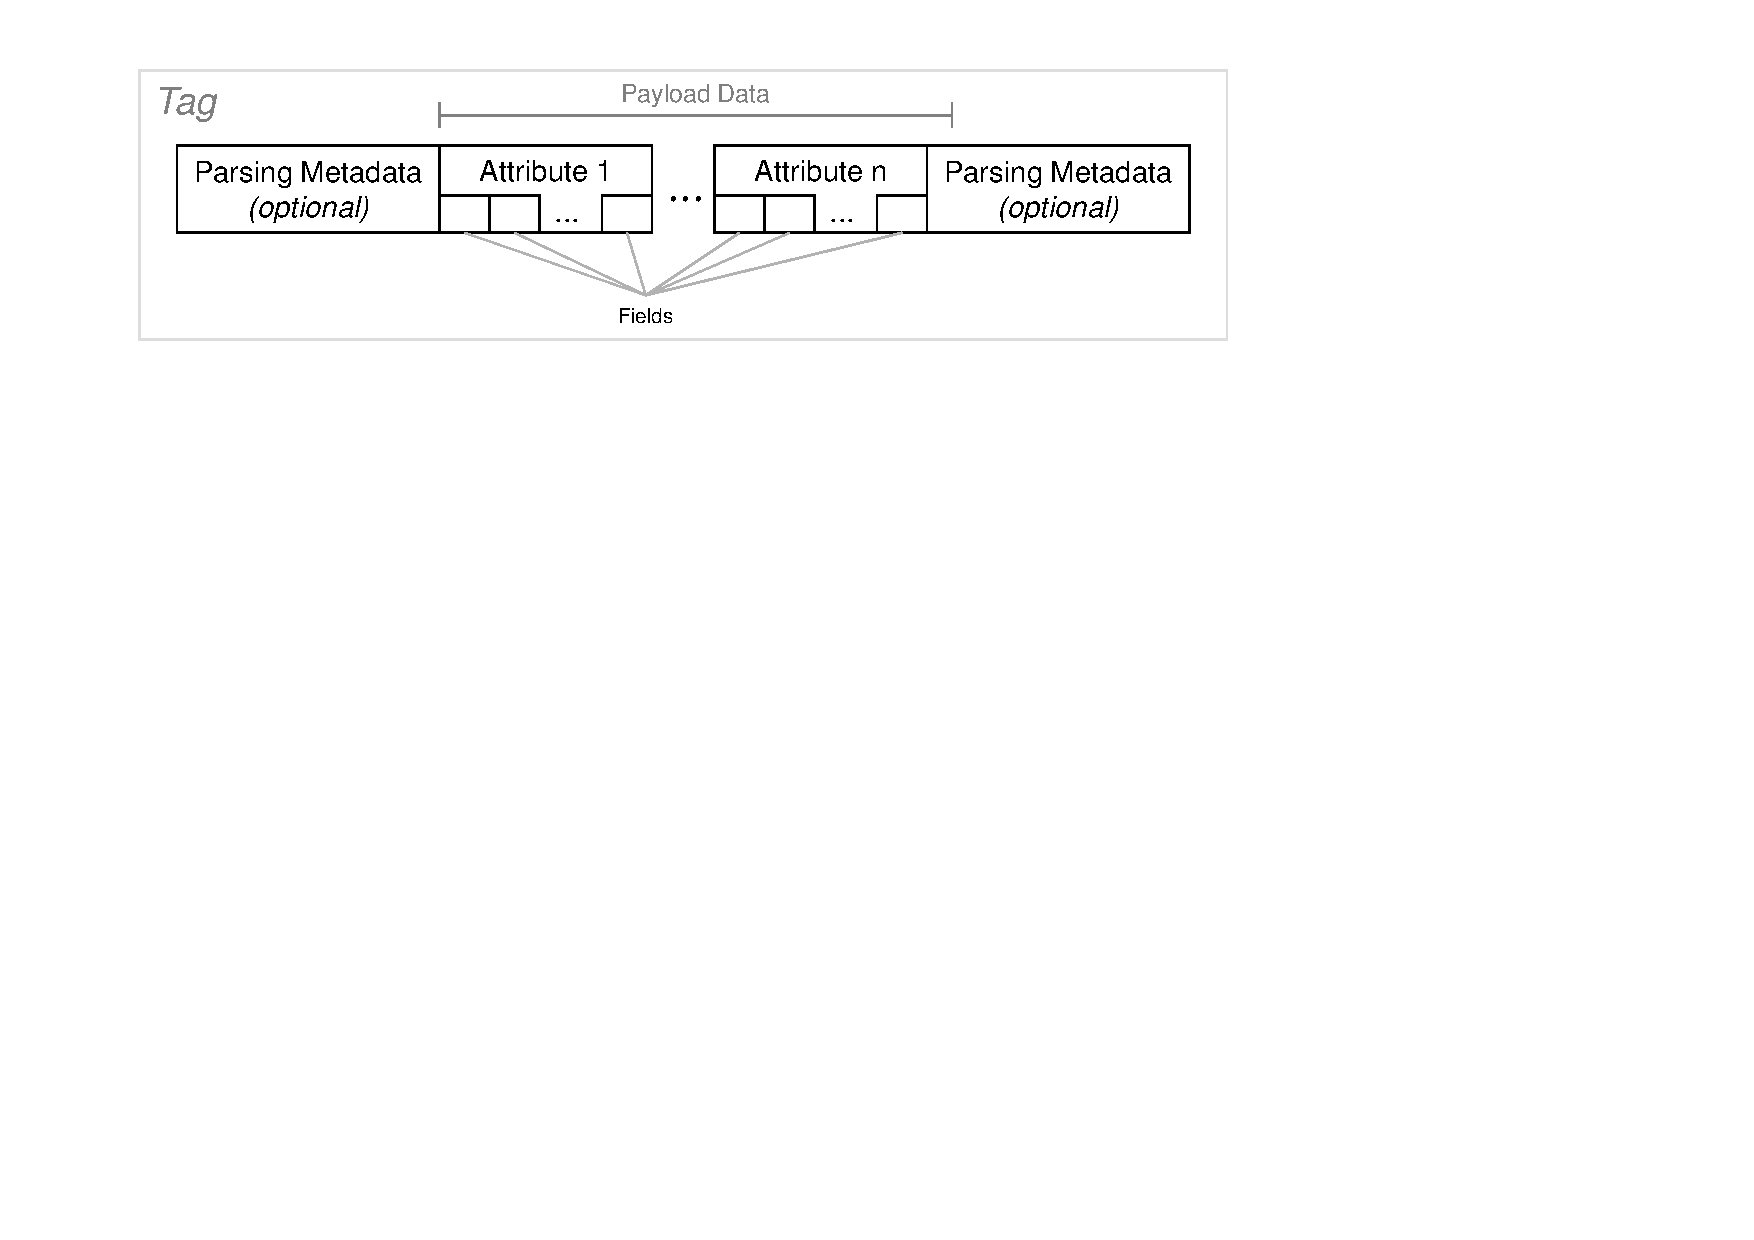
\includegraphics[width=1.00\textwidth]{Figures/Part_I/I_3_TagStructure.pdf}
		\caption{Struktur eines \TERMtag{}s}
	\label{fig:5_3_SCH_Tag}
\end{figure}

Die wichtigsten Teile eines \TERMtag{}s bilden die \TERMattribute{}e.

%***********************************************************************************************

\subsection{\TERMattribute{}}
\label{sec:Attribute}

Ein \TERMattribute{} ist ein Teil eines \TERMtag{}s, das die wertvollen Metadaten enth�lt als key-value-Paar enth�lt. Bekannte Beispiele sind K�nstler, Titel, Album, Komponist etc. eines Musikst�cks. H�ufig ist ein \TERMattribute{} auch ein \TERMcontainer{}, hat also ggf. einen \TERMheader{}, \TERMfooter{} und Nutzdaten. Der \TERMheader{} hilft meist dabei, den Typen (K�nstler, Title, oder Album) des \TERMattribute{} sowie die Gr��e von dessen Werte zu speichern. Die \TERMpayload{} enth�lt die jeweilige Information in einer kodierten Form, z.B. den Namen des K�nstlers oder Titels des Musikst�cks.

Die meisten \TERMattribute{}e haben nur einen unstrukturierten einfachen Wert. In manchen F�llen gibt es aber auch komplexer strukturierte \TERMattribute{}-Werte die aus mehreren Teilen in Form von Kind-\TERMfield{}ern oder gar \TERMdataBlocks{} bestehen.

In jedem Metadaten-Format hat ein \TERMattribute{} einen speziellen Namen, hier einige Beispiele:
\begin{itemize}
	\item ID3v1, Lyrics3: Field
	\item ID3v2: Frame
	\item APE: Item
	\item Matroska: SimpleTag
	\item VorbisComment: User Comment
\end{itemize}

In \TERMcontainerFormat{}en sind die \TERMattribute{}e h�ufig \TERMcontainer{} die im jeweiligen \TERMcontainerFormat{} definiert sind.

%***********************************************************************************************

\subsection{\TERMfield{}er}
\label{sec:Fields}

Ein \TERMfield{} ist eine Sequenz von Bits, die zusammen eine spezielle Bedeutung in einem gegebenen \TERMdataFormat{} haben. Das \TERMdataFormat{} beschreibt, wie ein spezieller \TERMdataBlock{} durch eine Folge von \TERMfield{}ern aufgebaut ist. Ein \TERMfield{} hat einen Wertebereich und es wird auch definiert, wie diese Werte jeweils zu interpretieren sind. Oft wird ein Teil des Wertebereiches als ``reserviert'' definiert, um eine gewisse Erweiterbarkeit des Datenformats sicherzustellen.

%-----------------------------------------------------------------------------------------------

\subsection{\TERMsubject{}}
\label{sec:Subject}

Ein \TERMsubject{} bezeichnet das Ding, das durch ein \TERMtag{} beschrieben wird, d.h. einen Teil einer Datei, oder eines Musikst�ckes, oder einer Web-Ressource or sogar eines real existierenden Objektes. H�ufig enth�lt ein \TERMtag{} Metadaten, die sich auf das aktuelle \TERMmedium{} als \TERMsubject{} beziehen, es wird nicht explizit auf ein spezielleres \TERMsubject{} referenziert.

%-----------------------------------------------------------------------------------------------

\section{\TERMmedium{}}
\label{sec:Medium}

Ein \TERMmedium{} bezeichnet Speichermedium der \TERMdataBlocks{}. Es kann sich dabei beispielsweise um eine Datei oder einen \TERMmediaStream{}, oder gar den Hauptspeicher selbst handeln.

%###############################################################################################
%###############################################################################################
%
%		File end
%
%###############################################################################################
%###############################################################################################